\begin{figure}[H]
	\centering
	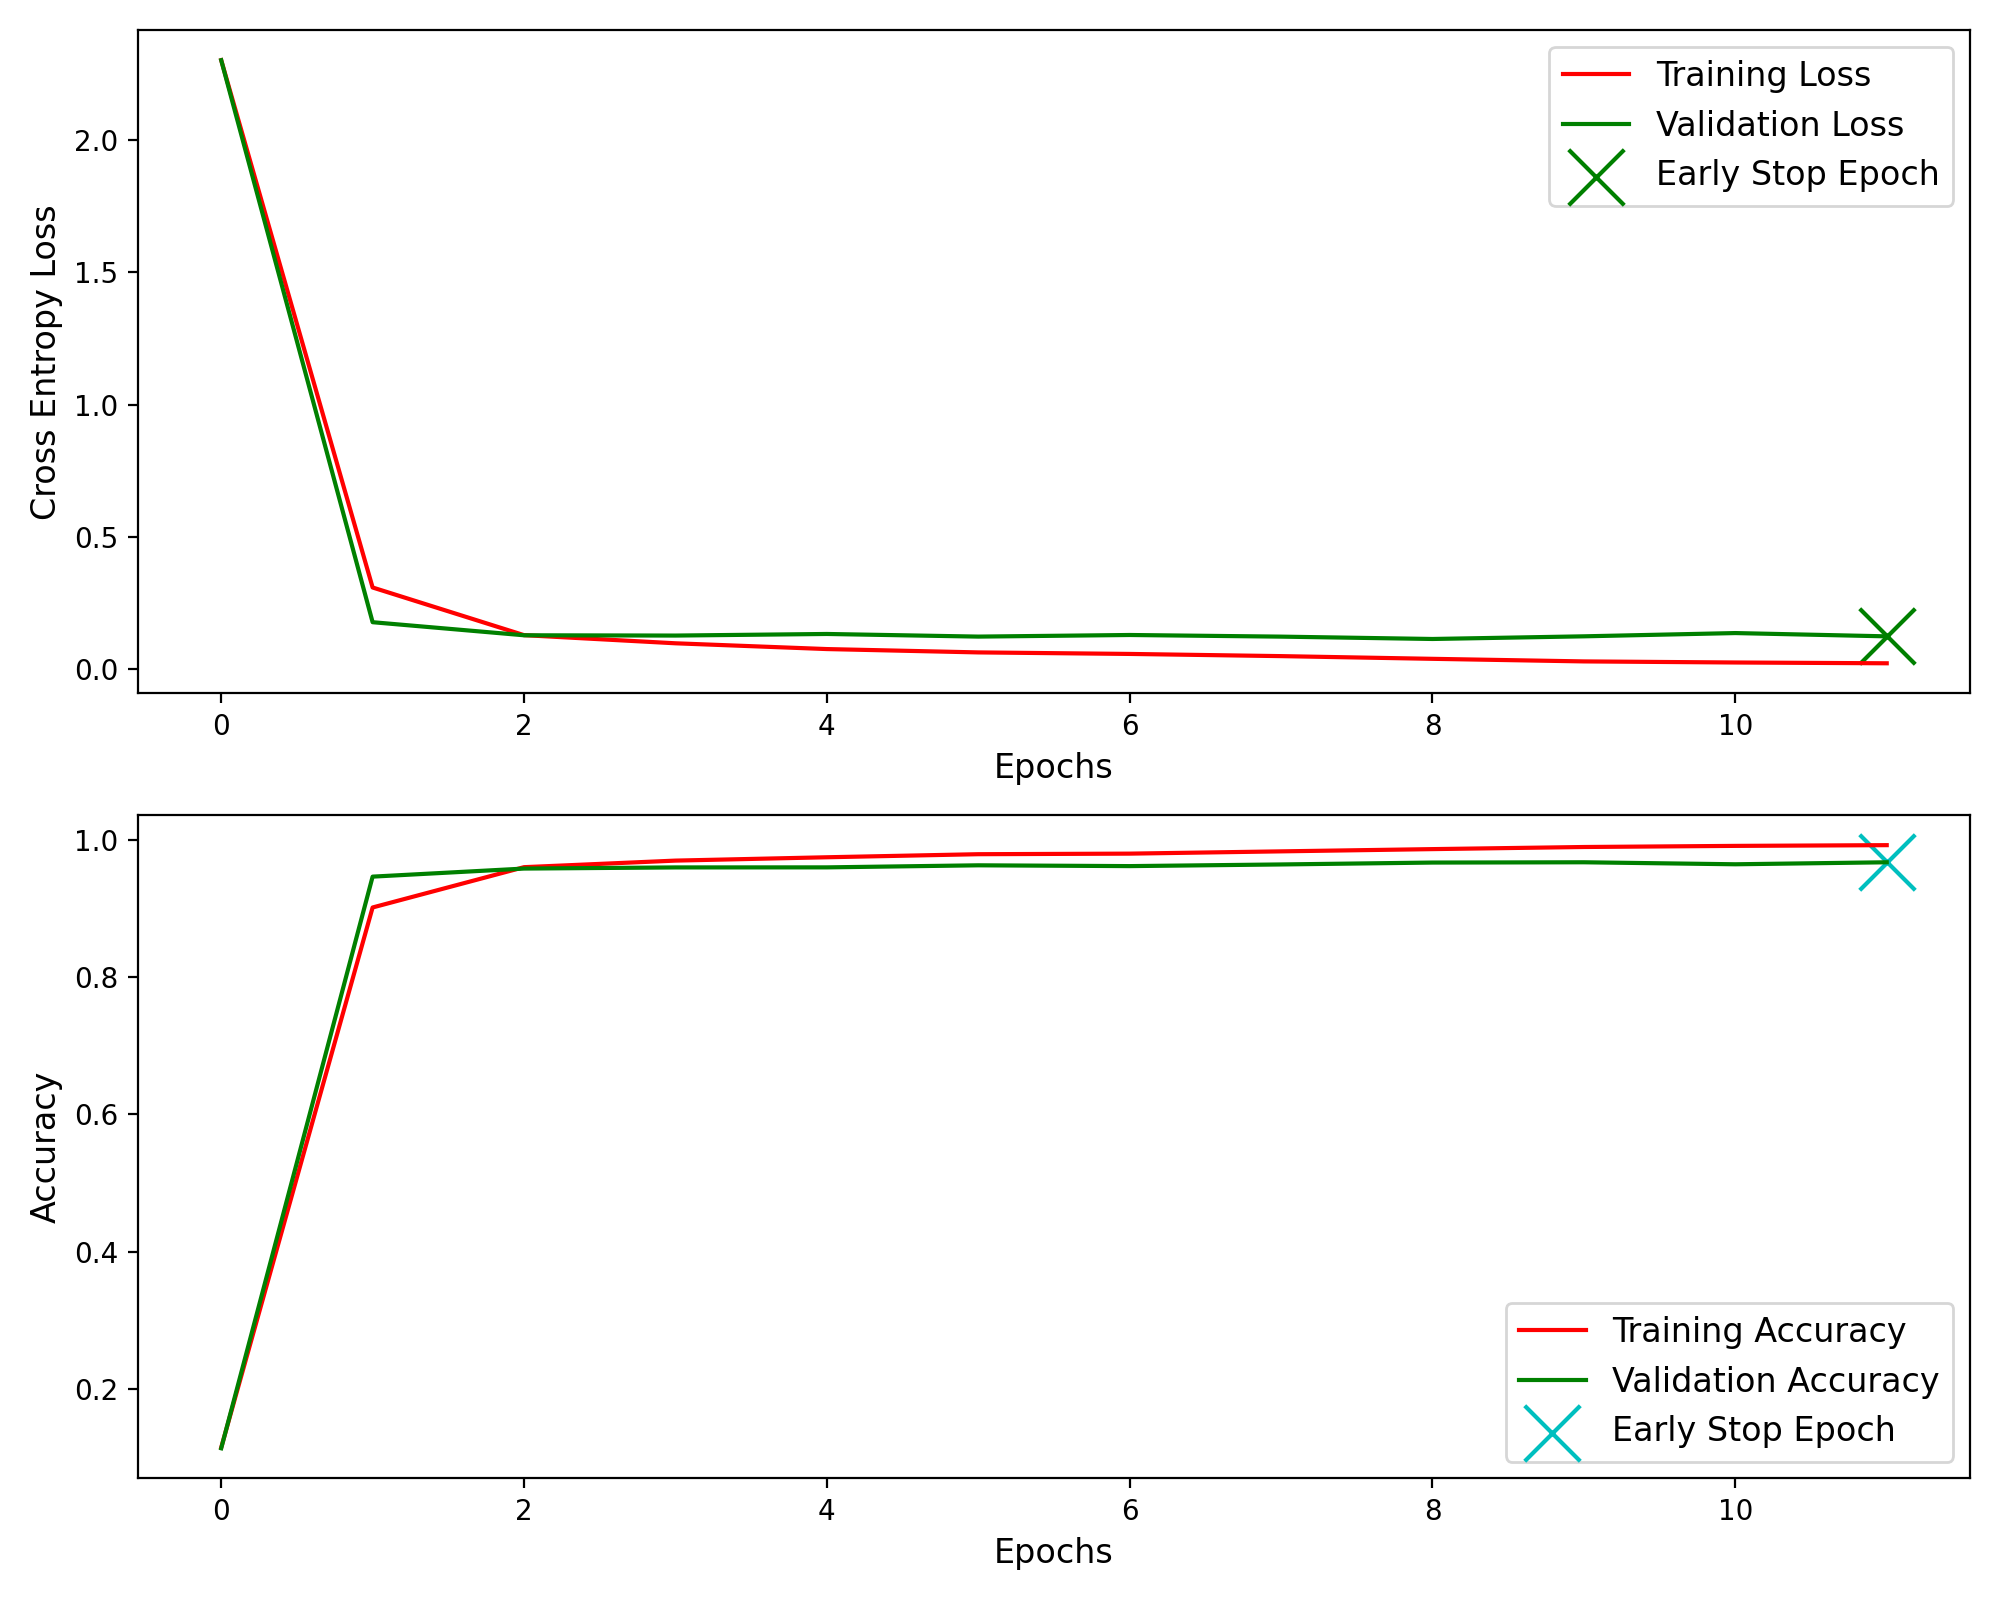
\includegraphics[width=1.0\textwidth]{./images/activation_tanh.png}
	\caption{Accuracy and Loss using $\tanh(x)$ activation}
	\label{fig:tanh}
\end{figure}


\begin{figure}[H]
	\centering
	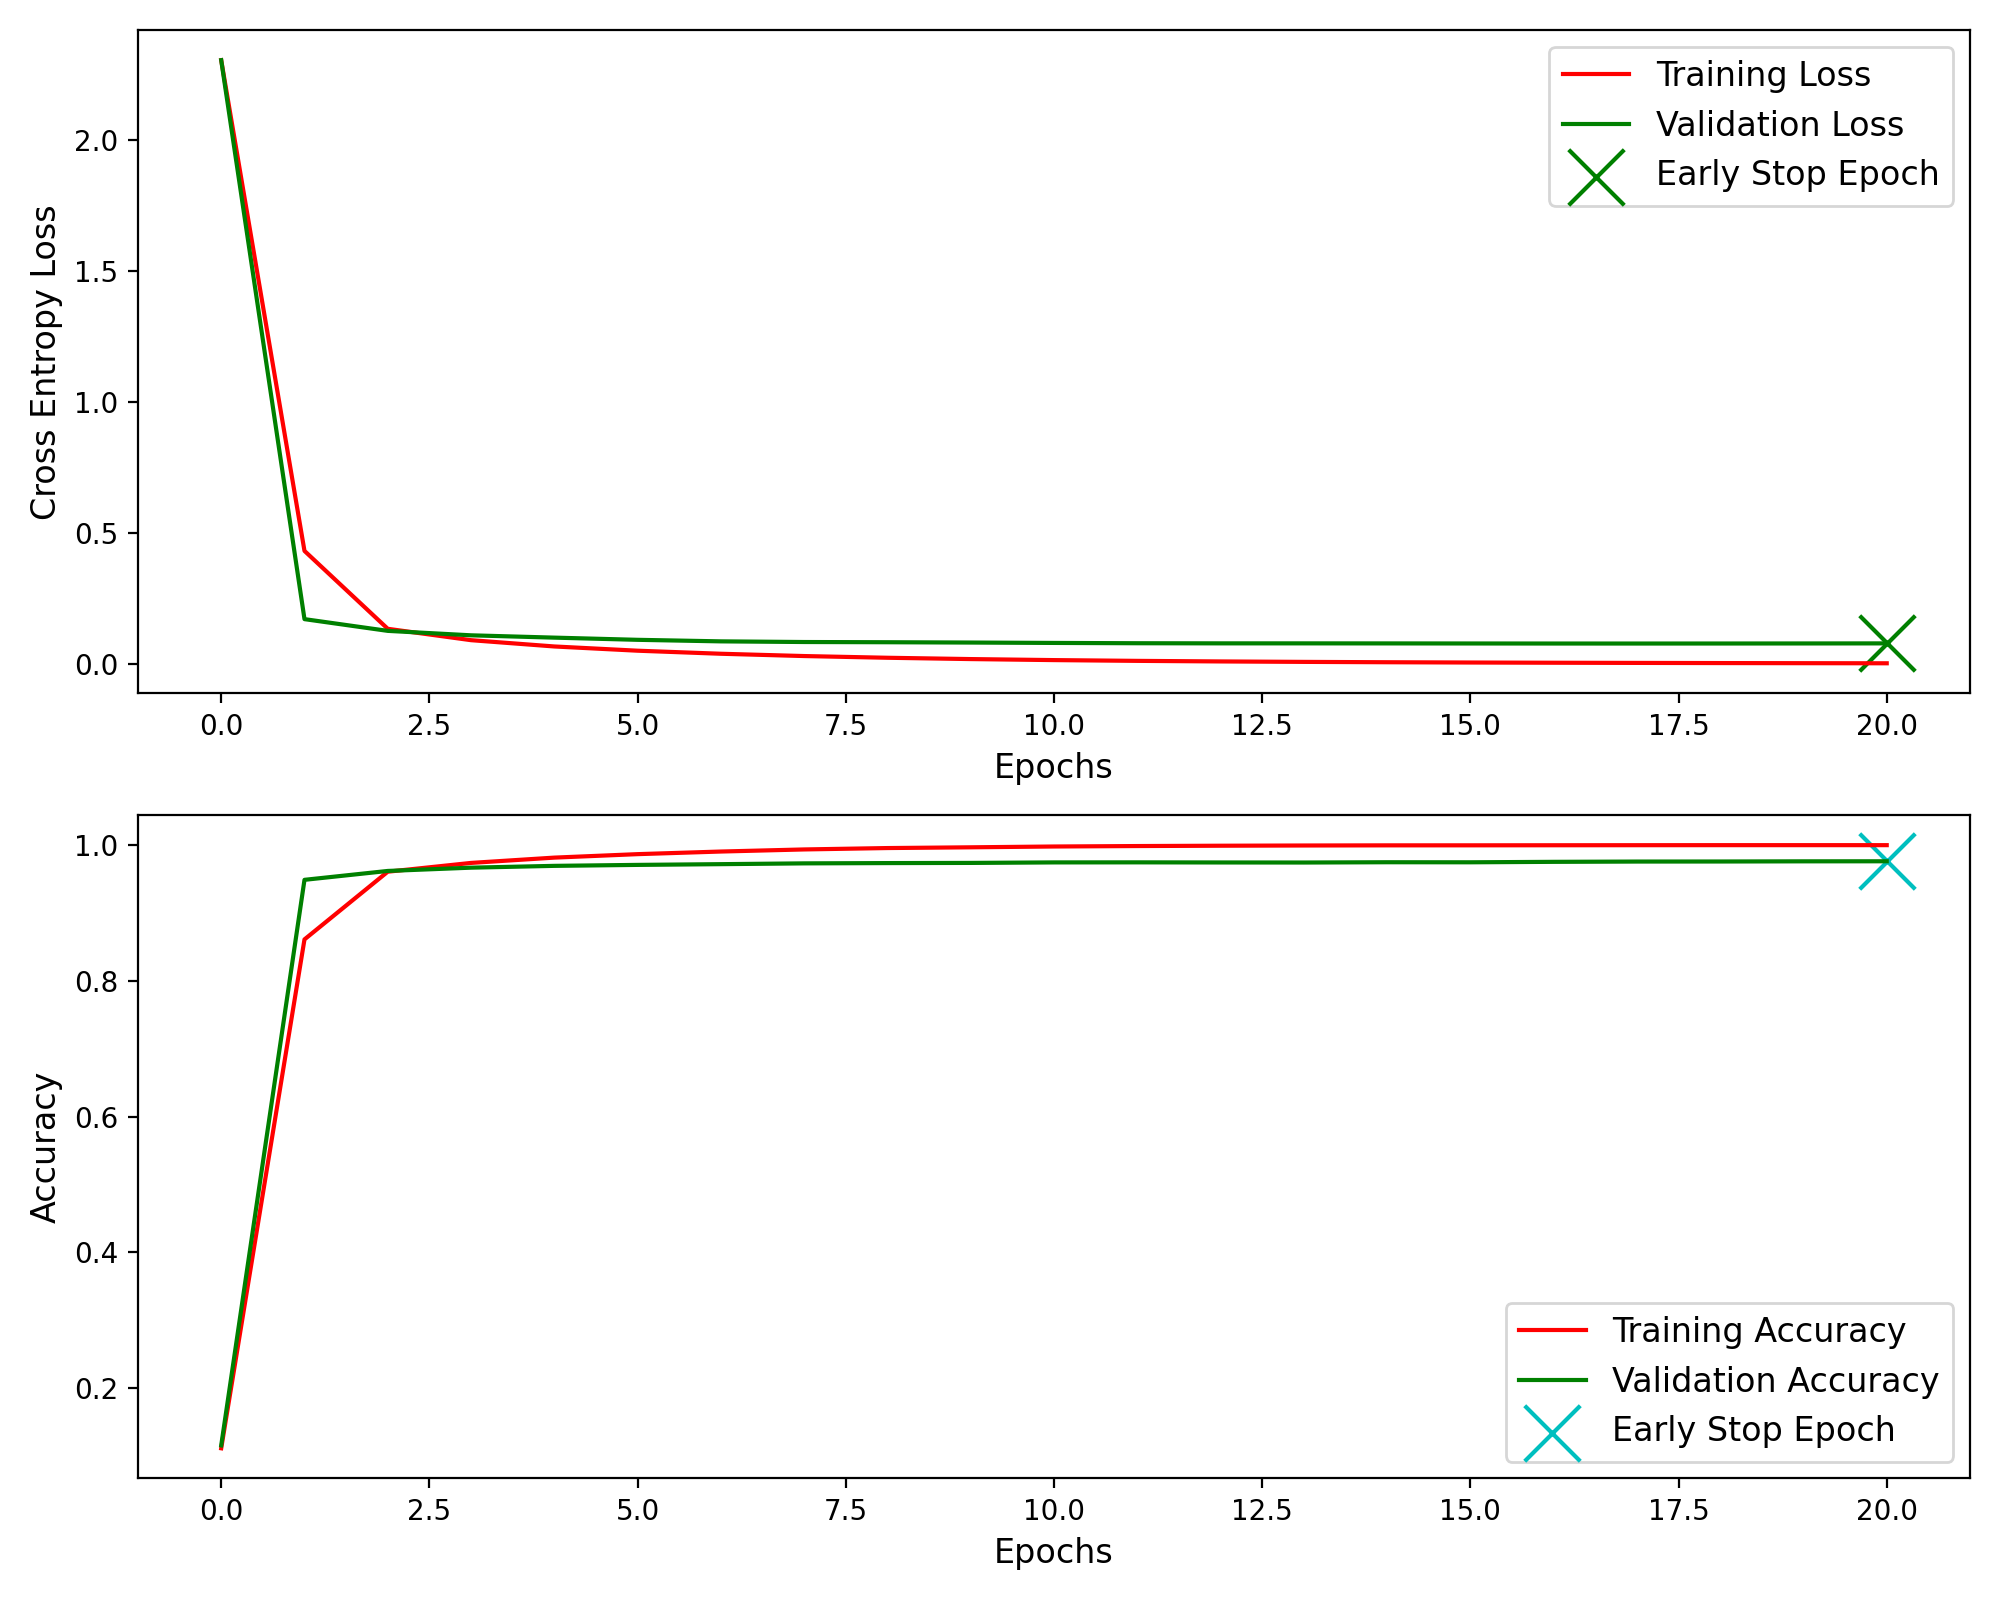
\includegraphics[width=1.0\textwidth]{./images/activation_sigmoid.png}
	\caption{Accuracy and Loss using $\texttt{sigmoid}(x)$ activation}
	\label{fig:sigmoid}
\end{figure}

\begin{figure}[H]
	\centering
	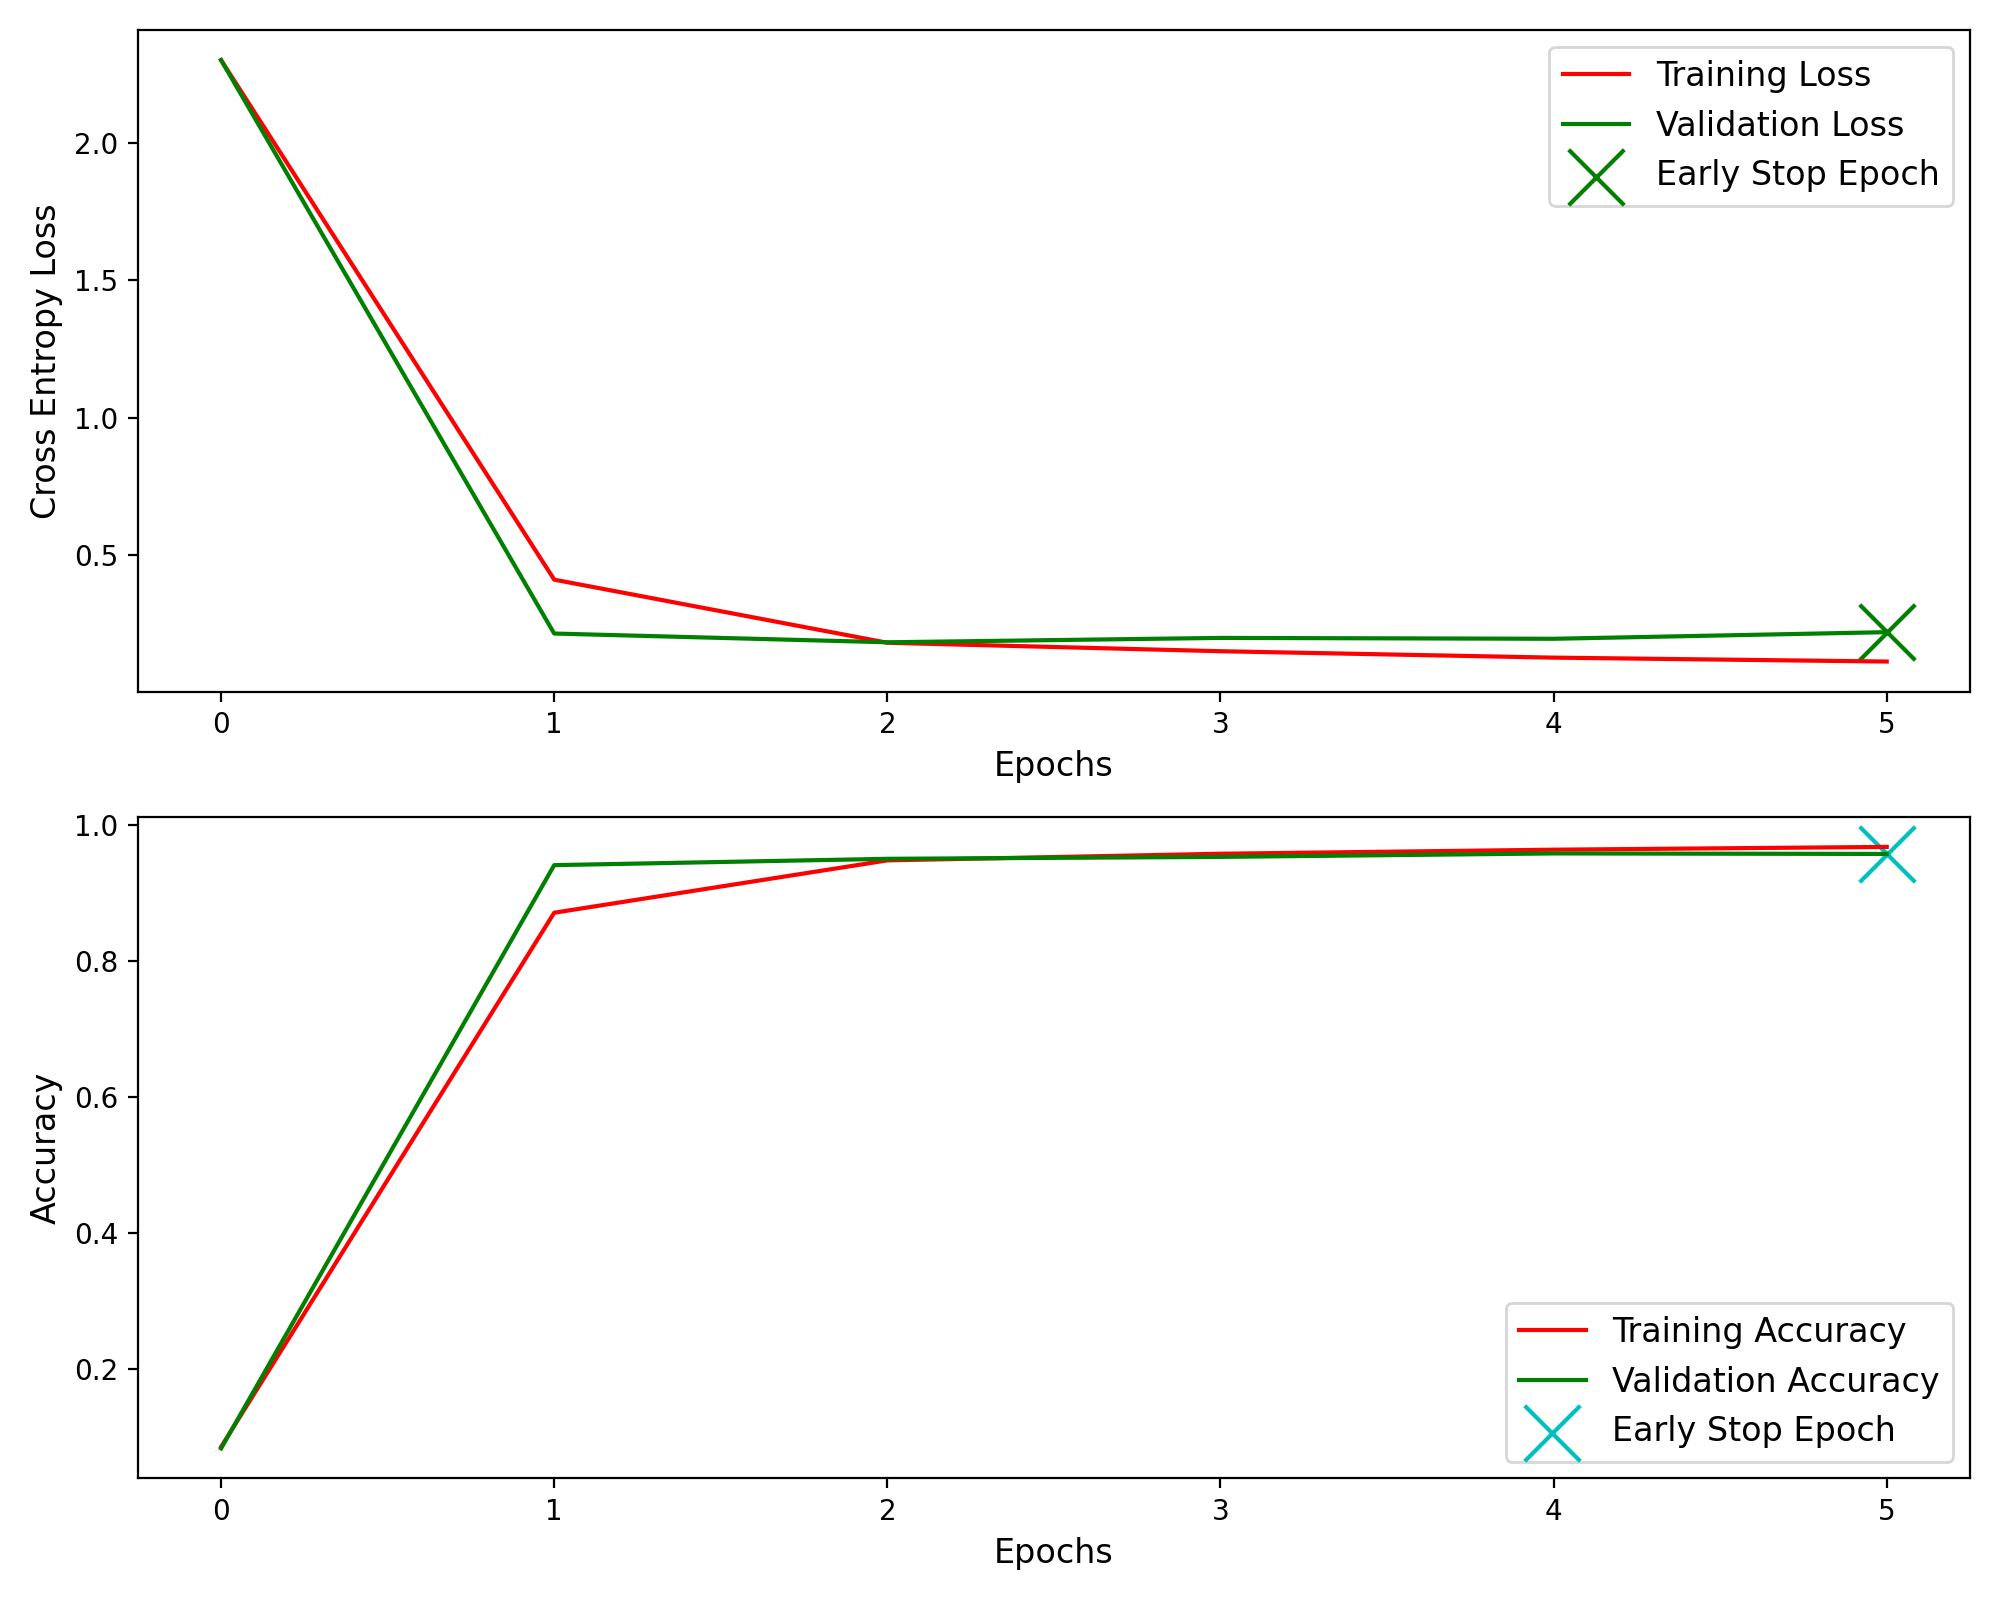
\includegraphics[width=1.0\textwidth]{./images/activation_relu.png}
	\caption{Accuracy and Loss using $\texttt{ReLU}(x)$ activation, $\alpha = 0.001$}
	\label{fig:relu}
\end{figure}

\begin{figure}[H]
	\centering
	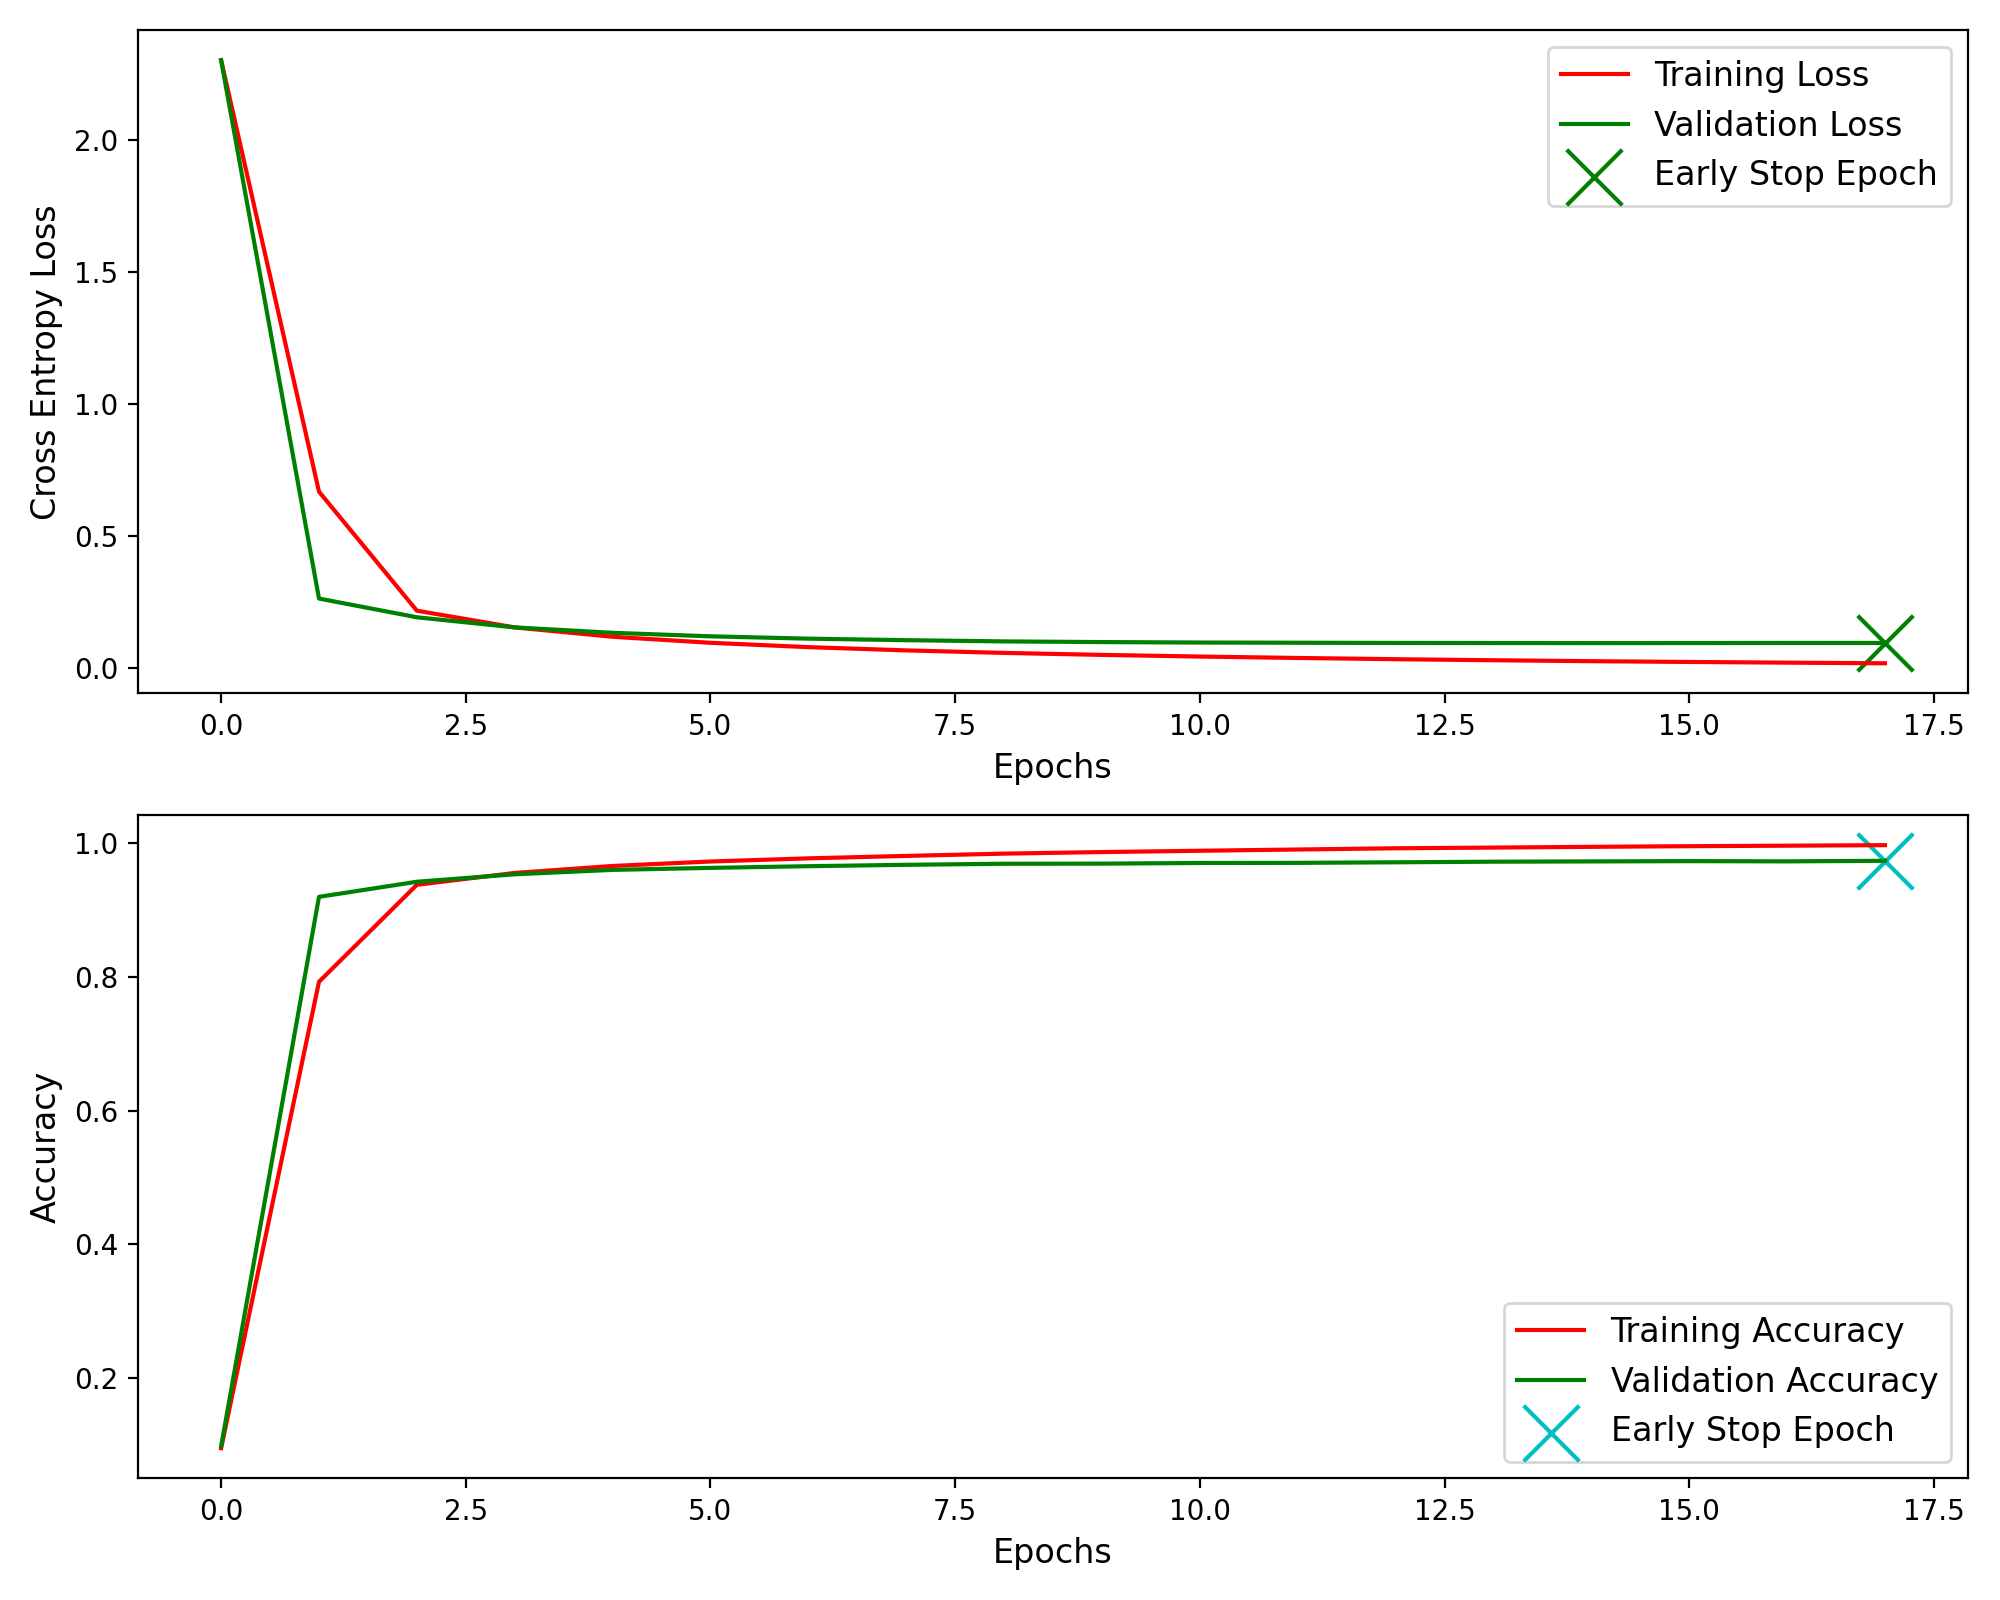
\includegraphics[width=1.0\textwidth]{./images/activation_relu2.png}
	\caption{Accuracy and Loss using $\texttt{ReLU}(x)$ activation, $\alpha = 0.0001$}
	\label{fig:relu2}
\end{figure}
\section{Activation Experiments}

\subsection{Background}

Neural networks utilize activation functions to introduce non-linearity into the model, enabling it to learn complex patterns and relationships in data. Three commonly used activation functions are \texttt{tanh}, \texttt{ReLU} (Rectified Linear Unit), and \texttt{sigmoid}.

\subsubsection{Tanh Activation Function}

The hyperbolic tangent function, \(\texttt{tanh}(x)\), is defined as:

\[
	\texttt{tanh}(x) = \frac{e^{x} - e^{-x}}{e^{x} + e^{-x}}
\]

The derivative of \(\texttt{tanh}(x)\) with respect to \(x\) is given by:

\[
	\frac{d}{dx} \texttt{tanh}(x) = 1 - \texttt{tanh}^2(x)
\]

Properties of \(\texttt{tanh}\):
\begin{itemize}
	\item Range: \([-1, 1]\)
	\item Zero-centered, which can aid in faster convergence during training.
\end{itemize}

\subsubsection{ReLU Activation Function}

The Rectified Linear Unit, \texttt{ReLU}(x), is defined as:

\[
	\texttt{ReLU}(x) = \max(0, x)
\]

The derivative of \texttt{ReLU}(x) is:

\[
	\frac{d}{dx} \texttt{ReLU}(x) = \begin{cases}
		0, & \text{if } x < 0    \\
		1, & \text{if } x \geq 0
	\end{cases}
\]

Properties of \texttt{ReLU}:
\begin{itemize}
	\item Simplicity and computationally efficient.
	\item Prone to the "dying ReLU" problem, where neurons can become inactive during training.
\end{itemize}

\subsubsection{Sigmoid Activation Function}

The sigmoid function, \(\texttt{sigmoid}(x)\), is defined as:

\[
	\texttt{sigmoid}(x) = \frac{1}{1 + e^{-x}}
\]

Its derivative is given by:

\[
	\frac{d}{dx} \texttt{sigmoid}(x) = \texttt{sigmoid}(x) \cdot (1 - \texttt{sigmoid}(x))
\]

Properties of \texttt{sigmoid}:
\begin{itemize}
	\item Output range: \((0, 1)\)
	\item Smooth gradient, facilitating gradient-based optimization.
	\item Susceptible to vanishing gradient problem.
\end{itemize}

\subsection{Performance}

We now consider the performance of our network with each activation function. We will
continue to use early stopping with $E = 3$, momentum with $\gamma = 0.9$, and $\alpha = 0.001$.
L1 and L2 normalization are not used.

\subsubsection{Tanh}

We get test accuracy of $97.15\%$ and a stopping epoch of $10$\cref{fig:tanh}.

\subsubsection{Sigmoid}


We get test accuracy of $97.66\%$ and a stopping epoch of $19$\cref{fig:sigmoid}.

\subsubsection{ReLU}

We get test accuracy of $95.61\%$ and a stopping epoch of $5$\cref{fig:relu}. The relatively
low performance and early stopping epoch suggests the learning rate is too high. If we set
$\alpha = 0.0001$, we get an accuracy of $97.56\%$ on the test data and stopping
epoch of $16$\cref{fig:relu2}.

\subsection{Observations}

With $\alpha = 0.001$ both sigmoid and tanh perform similarly on the test data, but
tanh converges much faster. ReLU performs fine, but poorly compared to the other two.
After seeing that ReLU was converging very fast, we tried reducing the learning rate
by a factor of 10. This brought ReLU's performance up to speed, but reduced its covergence time.
